In this section, we define the foundational objects of Computational Mechanics: causal states, the $\epsilon$-machine, and the primary measures of structure.

\subsection{Causal States and the $\epsilon$-Machine}
We consider a stationary stochastic process $\mathcal{P}$ producing a symbol sequence $\dots X_{-1}, X_0, X_1, \dots$ drawn from a finite alphabet $\mathcal{A}$. A \textit{history} $\overleftarrow{x}$ is a semi-infinite sequence of past observations.

The central premise of Computational Mechanics is that optimal prediction requires retaining only the information from the history that is statistically relevant for the future. We define the \textbf{causal equivalence relation} $\sim_{\epsilon}$ such that two histories are equivalent if and only if they have the same conditional distribution over futures \cite{shalizi2000computational}:
\begin{equation}
    \overleftarrow{x} \sim_{\epsilon} \overleftarrow{x}' \iff P(\vec{X} | \overleftarrow{X} = \overleftarrow{x}) = P(\vec{X} | \overleftarrow{X} = \overleftarrow{x}')
\end{equation}

The \textbf{Causal States} $\mathcal{S}$ are the equivalence classes induced by this relation. The \textbf{$\epsilon$-machine} is the unique, minimal unifilar hidden Markov model (HMM) defined by the causal states and their transitions. It captures the process's ``causal architecture.''

\subsection{Measures of Complexity}
The $\epsilon$-machine allows us to compute intrinsic properties of the process.

\subsubsection{Statistical Complexity ($C_\mu$)}
The statistical complexity is the amount of information about the past needed to optimally predict the future. It is the Shannon entropy of the causal state distribution $\pi$:
\begin{equation}
    C_\mu = H[\mathcal{S}] = - \sum_{\sigma \in \mathcal{S}} \pi(\sigma) \log_2 \pi(\sigma)
\end{equation}

\subsubsection{Entropy Rate ($h_\mu$)}
The entropy rate measures the irreducible randomness of the process per symbol. For a unifilar source, this is the average uncertainty of the next symbol given the current causal state:
\begin{equation}
    h_\mu = H[X|\mathcal{S}] = - \sum_{\sigma \in \mathcal{S}} \pi(\sigma) \sum_{x \in \mathcal{A}} P(x|\sigma) \log_2 P(x|\sigma)
\end{equation}

\subsection{Example: The Golden Mean Process}
To illustrate these concepts, we analyze the ``Golden Mean'' process. This process generates binary sequences where every $0$ must be followed by a $1$, but $1$s can be followed by $0$ or $1$ with equal probability ($p=0.5$).

\subsubsection{Inference}
We simulated a dataset ($N=100,000$) and used the CSSR algorithm via \texttt{emic} to infer the $\epsilon$-machine. The result is shown in Figure \ref{fig:gm_machine}.

\begin{figure}[H]
    \centering
    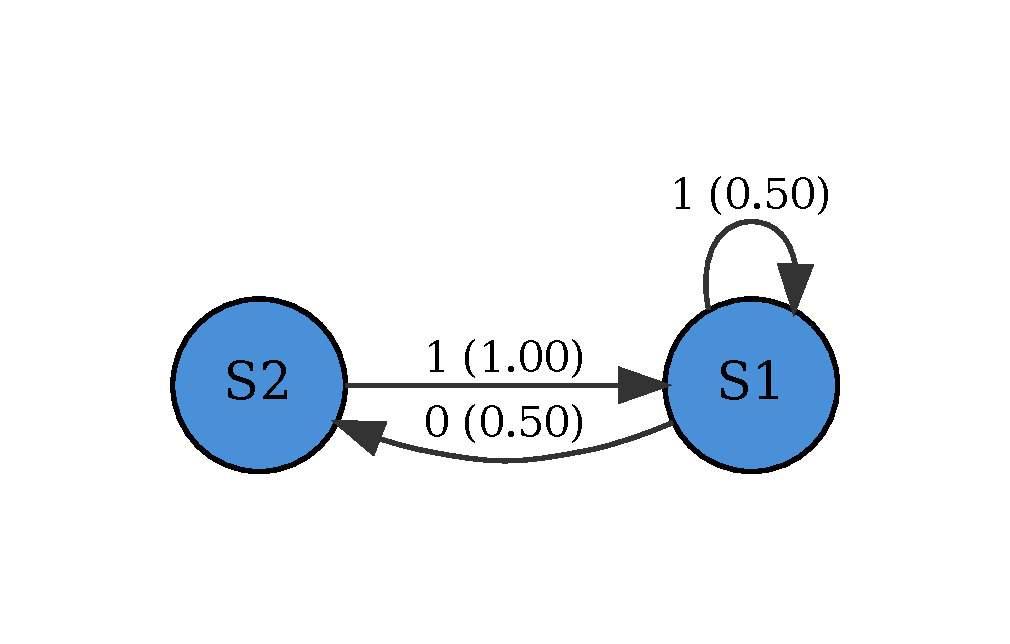
\includegraphics[width=0.6\textwidth]{figures/golden_mean_machine.pdf}
    \caption{The inferred $\epsilon$-machine for the Golden Mean process. Note the recovered structure matches the generator.}
    \label{fig:gm_machine}
\end{figure}

\subsubsection{Results}
Using the inferred machine, we compute the measures:
\begin{itemize}
    \item \textbf{States}: Two causal states are identified.
    \item \textbf{Stationary Distribution}:
    \begin{itemize}
    \item $P(A) \approx 0.665$
    \item $P(B) \approx 0.335$
\end{itemize}

    \item \textbf{Statistical Complexity}: $C_\mu \approx 0.918$ bits.
    \item \textbf{Entropy Rate}: $h_\mu \approx 0.667$ bits.
\end{itemize}
The theoretical values are $C_\mu \approx 0.918$ and $h_\mu = 2/3$, confirming the accuracy of the reconstruction.
